\documentclass[12pt,a4paper]{article}

% ====== PAKIETY ======
\usepackage[utf8]{inputenc}
\usepackage[T1]{fontenc}
\usepackage[polish]{babel}
\usepackage{lmodern}
\usepackage[a4paper,margin=2.5cm]{geometry}
\usepackage{graphicx}
\usepackage{float}
\usepackage{xcolor}
\usepackage{titlesec}
\usepackage{enumitem}
\usepackage{booktabs}
\usepackage{tabularx}
\usepackage{longtable}
\usepackage{seqsplit}
\usepackage{listings}
\usepackage{hyperref}
\usepackage{microtype}
\usepackage[utf8]{inputenc}
\usepackage[polish]{babel}

\setlength{\emergencystretch}{3em}


% ====== LINKI ======
\hypersetup{
  colorlinks=true,
  linkcolor=black,
  urlcolor=teal,
  citecolor=black
}


\lstset{
	basicstyle=\ttfamily\footnotesize,
	keywordstyle=\color{blue}\bfseries,
	commentstyle=\color{gray}\itshape,
	stringstyle=\color{orange!80!black},
	numbers=left,
	numberstyle=\tiny\color{gray},
	stepnumber=1,
	breaklines=true,
	frame=single,
	rulecolor=\color{black!30},
	backgroundcolor=\color{gray!8},
	captionpos=b,
	showstringspaces=false,
	tabsize=4,
	extendedchars=true,
	literate={ą}{{\k{a}}}1 {ć}{{\'c}}1 {ę}{{\k{e}}}1 {ł}{{\l{}}}1 {ń}{{\'n}}1 {ó}{{\'o}}1 {ś}{{\'s}}1 {ź}{{\'z}}1 {ż}{{\.z}}1
	{Ą}{{\k{A}}}1 {Ć}{{\'C}}1 {Ę}{{\k{E}}}1 {Ł}{{\L{}}}1 {Ń}{{\'N}}1 {Ó}{{\'O}}1 {Ś}{{\'S}}1 {Ź}{{\'Z}}1 {Ż}{{\.Z}}1
	{α}{{$\alpha$}}1 {·}{{$\cdot$}}1 
}
\renewcommand{\lstlistingname}{Kod}

% ====== METADANE ======
\begin{document}
	
	\begin{titlepage}
		\centering
		\vspace*{2cm}
		
		{\Large \textbf{Politechnika Białostocka} \par}
		{\large Wydział Informatyki \par}
		
		\vspace{3.5cm}
		
		{\Huge \textbf{Finansista PB} \par}
		\vspace{0.8cm}
		{\Large System obsługi wniosków o finansowanie \\ działalności studenckiej i doktoranckiej \par}
		
		\vspace{2.5cm}
		
		{\Large \textbf{Dokumentacja projektowa} \par}
		
		\vspace{2.5cm}
		
		{\large \textbf{Autorzy:} \par}
		\vspace{0.2cm}
		{\large Jakub Matusiewicz \par}
		{\large Jakub Borkowski \par}
		{\large \textbf{Prowadzący:} \par}
		\vspace{0.2cm}
		{\large inż. Adrian Twardowski \par}
		\vspace{0.8cm}
		{\small Przedmiot: Programowanie Aplikacji WWW w języku Java \par}
		\vspace{0.3cm}
		{\small Repozytorium: \url{https://github.com/kubus2731/finansista} \par}

		\vfill
		
		{\large Białystok, 19 czerwca 2026 \par}
	\end{titlepage}
	
	\thispagestyle{empty}
	\newpage
	
	\tableofcontents
	\newpage
% ====================================================================
\section{Wstęp}
\label{sec:wstep}

\subsection{Cel projektu}
Celem projektu jest dostarczenie systemu informatycznego usprawniającego proces
składania, oceny i rozliczania wniosków o finansowanie działalności studenckiej
i doktoranckiej w Politechnice Białostockiej. System realizuje papierowy obieg
wniosku opisany w \emph{Zarządzeniu nr 13/2025 Rektora Politechniki Białostockiej
z dnia 14 lutego 2025 r. w sprawie wydatkowania środków finansowych przeznaczonych
na działalność studencką i doktorancką}, ze szczególnym uwzględnieniem
\emph{Załącznika nr 1} (wzór formularza wniosku).

\subsection{Zakres}
System obejmuje:
\begin{itemize}[leftmargin=*]
  \item rejestrację oraz logowanie użytkowników z rozróżnieniem ról,
  \item składanie wniosku w wersji elektronicznej w pełni odwzorowującej Załącznik nr 1,
  \item walidację formularza (pola obowiązkowe, spójność dat i kwot, suma źródeł finansowania),
  \item obieg statusów wniosku (maszyna stanów po stronie bazy danych),
  \item podgląd statusu i szczegółów wniosku przez wnioskodawcę,
  \item REST API jako warstwę komunikacji frontend--backend,
  \item dokumentację OpenAPI dla wystawionych usług,
  \item logikę składowaną w bazie danych (pakiety, widoki, wyzwalacze, funkcje),
  \item zgodność z wymaganiami dostępności (deklaracja dostępności).
\end{itemize}

\section{Wymagania}
\label{sec:wymagania}

\subsection{Wymagania funkcjonalne}
\begin{enumerate}[leftmargin=*]
  \item Rejestracja i logowanie użytkownika.
  \item Wypełnianie wniosku poprzez formularz odwzorowujący Załącznik nr 1.
  \item Walidacja formularza.
  \item Wysyłanie wniosku do wyższych jednostek (zmiana statusu DRAFT $\to$ SUBMITTED).
  \item Kontrola wniosku finansowego poprzez sprawdzanie jego statusu.
  \item Edycja/poprawa wniosku w razie odrzucenia lub uwag.
  \item Procedowanie wniosku przez wyższe jednostki (Dziekanat, CSSDiR, Kwestor) - pola
        dostępne dla odpowiednich ról oraz odpowiednie ścieżki dla konkretnych wniosków.
  \item Dostępność aplikacji dla osób ze specjalnymi potrzebami.
  \item Filtrowanie i wyszukiwanie wniosków.
  \item Zarządzanie uprawnieniami i rolami użytkowników (administrator).
  \item Wyświetlanie pełnej historii zmian statusu wniosku.
  \item Źródło finansowania jako zmienna w encji wniosku.
\end{enumerate}

\subsection{Wymagania niefunkcjonalne}
\begin{itemize}[leftmargin=*]
  \item \textbf{Architektura}: klient--serwer; frontend i backend to
        \emph{osobne moduły Maven} uruchamiane jako niezależne procesy
        Spring Boot (frontend port 8081, backend port 8080). Komunikacja
        wyłącznie poprzez REST API z tokenem JWT.
  \item \textbf{Wydajność}: poprawna praca przy zbiorach 1\,000--1\,000\,000 wniosków
        (z paginacją i odpowiednimi indeksami).
  \item \textbf{Bezpieczeństwo}: uwierzytelnianie tokenem JWT przechowywanym w bezpiecznym
        ciasteczku \texttt{HttpOnly}, autoryzacja oparta na rolach.
  \item \textbf{Dostępność}: zgodność z WCAG 2.1 - skip link, semantyczne nagłówki,
        kontrast, etykiety formularzy, opublikowana deklaracja dostępności.
\end{itemize}


\section{Architektura systemu}
\label{sec:architektura}

System jest aplikacją o architekturze \textbf{multi-module} -- frontend
i backend są \emph{osobnymi modułami Maven}, uruchamianymi jako dwa
niezależne procesy Spring Boot na różnych portach. To fizyczna realizacja
wymagania ,,frontend działa niezależnie od backendu'' z deklaracji projektowej.

\begin{itemize}[leftmargin=*]
  \item \textbf{Moduł \texttt{frontend}} (port \texttt{8081}) -- aplikacja
        Spring Boot z kontrolerami Spring MVC zwracającymi widoki Thymeleaf,
        spakowana jako uruchamialny JAR (\texttt{finansista-frontend}).
        Frontend \emph{nie korzysta} z warstwy biznesowej ani repozytoriów
        backendu -- komunikuje się z nim wyłącznie przez HTTP poprzez
        \texttt{RestClient} (klasa \texttt{RestClientConfig}, baseUrl
        \texttt{app.backend.url}), przekazując token JWT pobrany z ciasteczka
        przeglądarki jako nagłówek \texttt{Authorization: Bearer}.
  \item \textbf{Moduł \texttt{backend}} (port \texttt{8080}) -- aplikacja
        Spring Boot wystawiająca REST API pod \texttt{/api/v1/**} (JSON).
        Zawiera całą logikę domenową (use case'y), warstwę dostępu do bazy
        (Spring Data JPA), bezpieczeństwo (Spring Security + JWT) oraz
        specyfikację OpenAPI (Swagger UI).
  \item \textbf{Warstwa danych} -- Oracle Database 23ai Free z migracjami
        Flyway, logiką składowaną (PL/SQL: pakiety, widoki, wyzwalacze)
        i dostępem przez JPA/Hibernate.
\end{itemize}

\paragraph{Struktura Maven}
Root projektu (\texttt{pom.xml} w katalogu głównym) ma typ \texttt{pom}
(\emph{parent}) i agreguje dwa moduły:
\texttt{<module>backend</module>} i \texttt{<module>frontend</module>}.
Moduł \texttt{frontend} jest w pełni niezależny -- jego \texttt{pom.xml}
nie zawiera zależności na \texttt{finansista-backend} i korzysta wyłącznie
ze starterów Spring Boot (web, thymeleaf, security, validation) oraz
Jackson i Lombok. Klasy DTO używane w komunikacji HTTP
(\texttt{CreateRequestRequest}, \texttt{RequestResponse} itp.) są
zdefiniowane po stronie frontendu (pakiet
\texttt{...frontend.viewmodel}), niezależnie od ich odpowiedników
w backendzie. Dzięki temu frontend może zostać wydzielony do osobnego
repozytorium (np.\ jako aplikacja SPA) bez zmian w kodzie.

\subsection{Stos technologiczny}
\begin{itemize}[leftmargin=*]
  \item Java 25, Spring Boot 4.0
  \item Spring MVC, Thymeleaf 3, Bootstrap 5
  \item Spring Security, JJWT 0.12
  \item Hibernate / Spring Data JPA
  \item Flyway (migracje)
  \item Oracle Database 23 Free (kontener Docker)
  \item Lombok, springdoc-openapi 3.0.3 (Swagger UI / OpenAPI 3.1)
  \item Build: Maven
\end{itemize}

\section{Model danych}
\label{sec:model-danych}

\subsection{Diagram encji}
\begin{figure}[H]
  \centering
  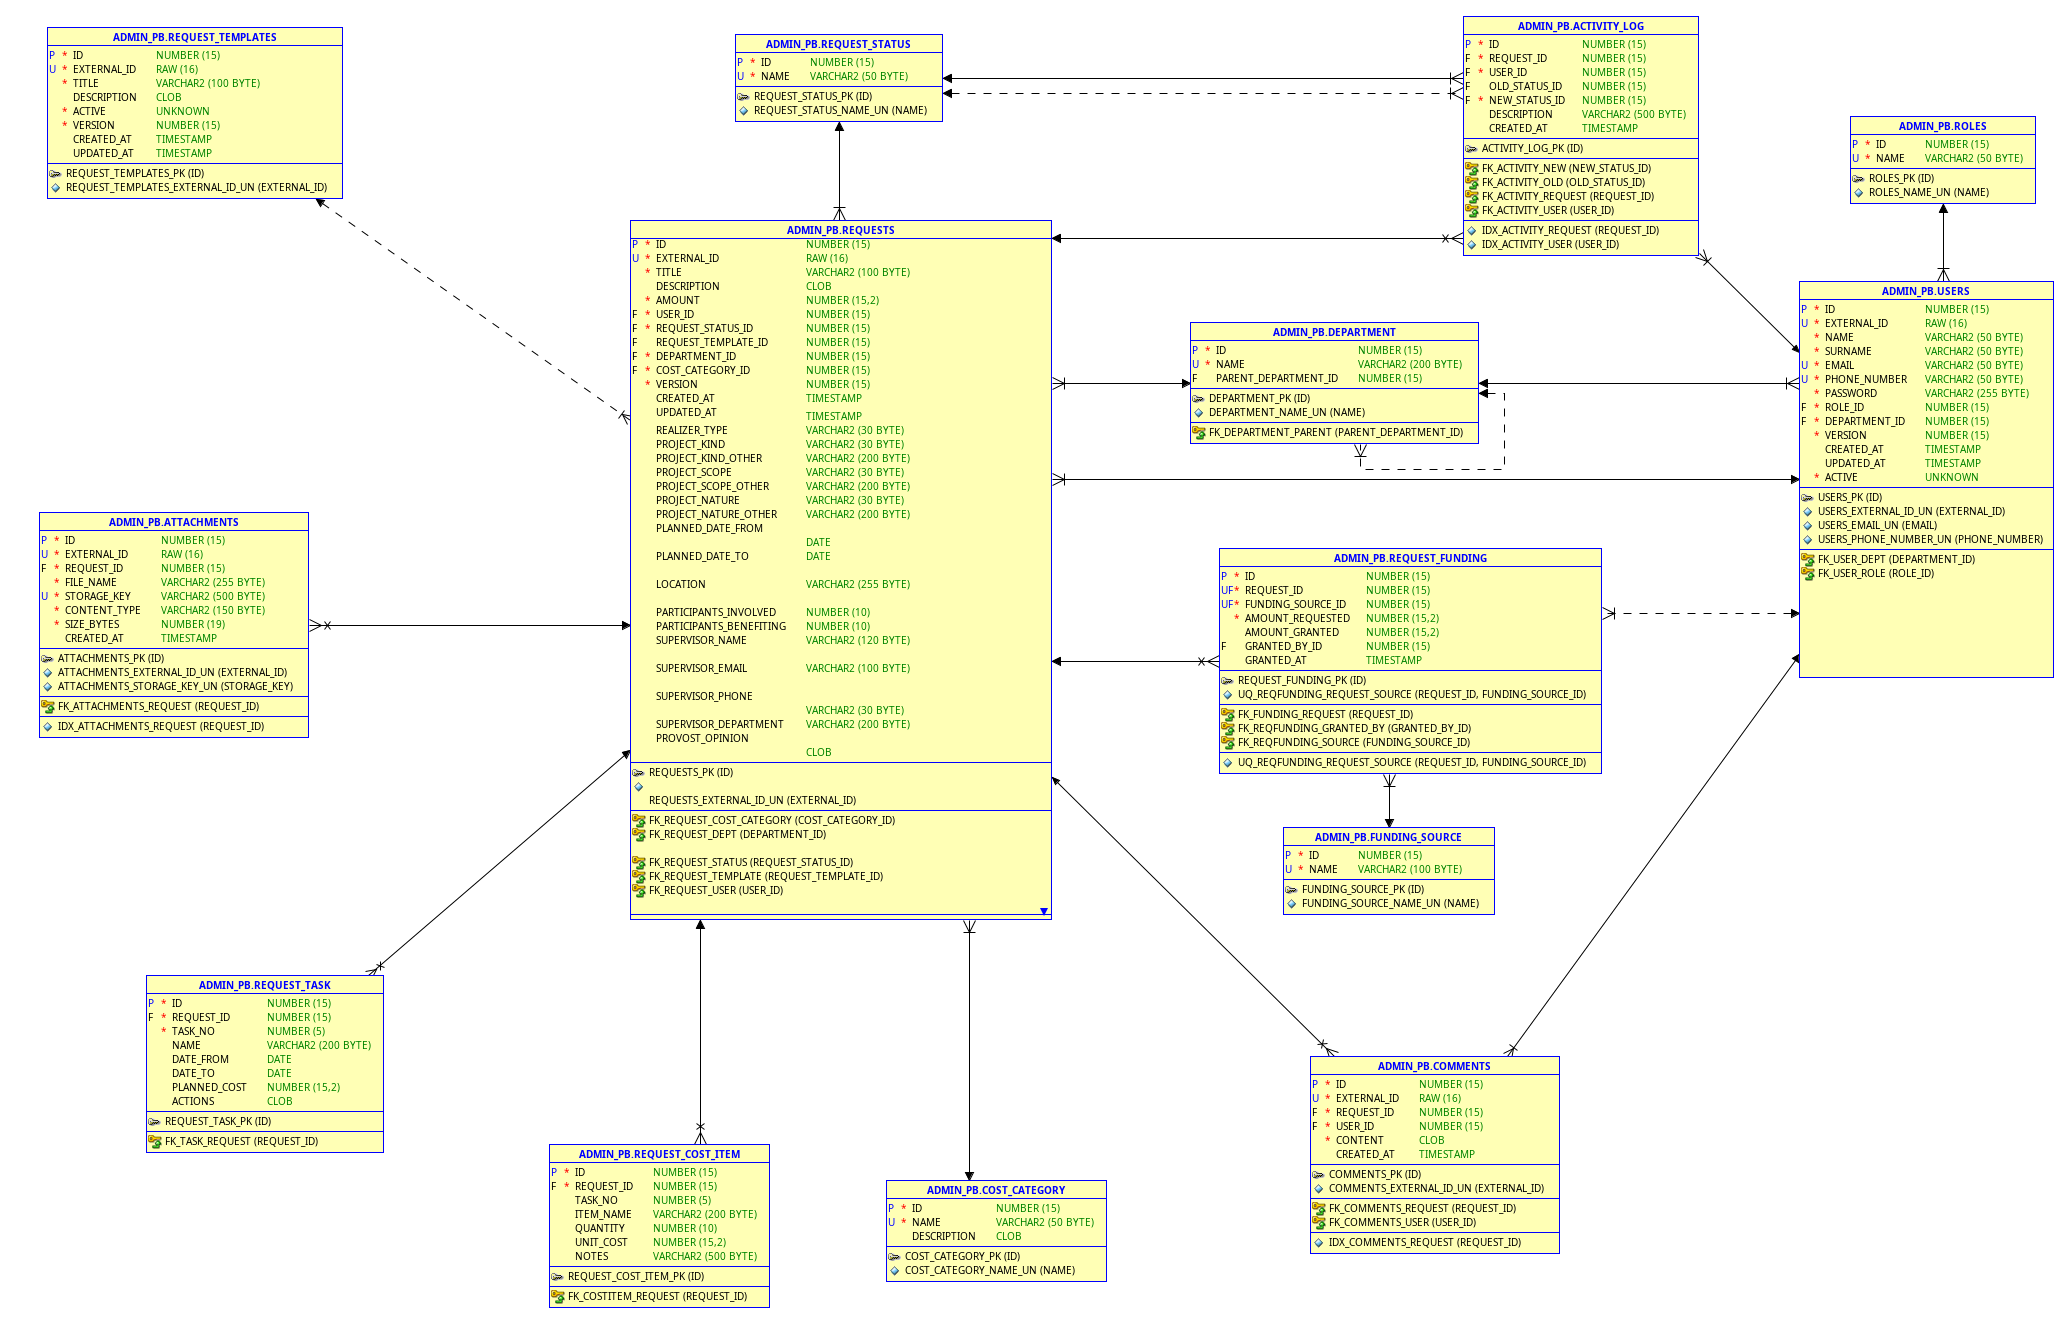
\includegraphics[width=\textwidth]{diagram_encji.png}
  \caption{Diagram encji}
  \label{fig:erd}
\end{figure}

\subsection{Główne tabele}
\begin{itemize}[leftmargin=*]
  \item \texttt{users} - konta użytkowników; powiązane z \texttt{roles} i \texttt{department}.
  \item \texttt{requests} - główna encja wniosku (sekcje I--III Załącznika nr 1).
        Tabela zawiera komplet pól Załącznika (typ realizatora, rodzaj/zakres/charakter
        projektu wraz z polami \emph{,,inne''}, daty planowanego przedsięwzięcia,
        liczby uczestników, dane opiekuna naukowego).
  \item \texttt{request\_task} - pozycje harmonogramu (sekcja IV).
  \item \texttt{request\_cost\_item} - pozycje kosztorysu (sekcja IV).
  \item \texttt{request\_funding} - \textbf{multi-source funding}: wniosek może
        być finansowany z \emph{wielu} źródeł równocześnie (Samorząd, Inicjatywy,
        Środki Wydziału\ldots), każde z osobną kwotą wnioskowaną
        (\texttt{amount\_requested}) i przyznaną (\texttt{amount\_granted}).
        Para (\texttt{request\_id}, \texttt{funding\_source\_id}) jest unikalna.
  \item \texttt{request\_status} - słownik statusów wniosku.
  \item \texttt{activity\_log} - historia zmian statusu (zasilana przez trigger \texttt{T\_ACTIVITY}).
  \item \texttt{comments}, \texttt{attachments} -- komentarze i załączniki do wniosków.
  \item Słowniki: \texttt{roles}, \texttt{department}, \texttt{cost\_category},
        \texttt{funding\_source}, \texttt{request\_templates}.
\end{itemize}

\subsection{Wartości osadzone (\emph{JPA Embeddables})}
Pola Załącznika nr 1 fizycznie żyją w tabeli \texttt{requests} (płaski schemat),
ale w warstwie obiektowej zostały zgrupowane w \textbf{value objects} przy
pomocy adnotacji \texttt{@Embeddable} -- wzorzec znany z \emph{Domain-Driven
Design}. Zapewnia to czytelność modelu (mniej pól w \texttt{Request}, jasna
semantyka), zachowując wydajność (brak dodatkowych \texttt{JOIN}-ów):

\begin{itemize}[leftmargin=*]
  \item \texttt{ProjectDetails} - sekcja I Załącznika: \texttt{realizerType},
        \texttt{projectKind}\slash\texttt{projectKindOther},
        \texttt{projectScope}\slash\texttt{projectScopeOther},
        \texttt{projectNature}\slash\texttt{projectNatureOther},
        \texttt{plannedDateFrom}\slash\texttt{plannedDateTo}, \texttt{location},
        \texttt{participantsInvolved}, \texttt{participantsBenefiting}.
  \item \texttt{SupervisorInfo} -- sekcja II Załącznika: dane opiekuna
        naukowego (imię i nazwisko, e-mail, telefon, jednostka).
\end{itemize}

Klasy te są niemutowalne (\texttt{@NoArgsConstructor(access = PROTECTED)} +
konstruktor z wszystkimi polami), eksponują jedynie gettery i mają fabrykę
\texttt{empty()} dla wniosku w trakcie tworzenia.

\subsection{Klucze hybrydowe}
Każda eksponowana encja używa dwóch identyfikatorów:
wewnętrznego \texttt{id} (\texttt{NUMBER IDENTITY}) używanego w kluczach obcych
oraz zewnętrznego \texttt{external\_id} (\texttt{RAW(16)} -- UUID v7),
który jest jedynym identyfikatorem wystawianym w REST API i adresach URL.
Zapobiega to wycieksowi informacji o liczności rekordów i utrudnia enumerację zasobów.

\subsection{Migracje Flyway}
Schemat bazy danych budowany jest sekwencją migracji Flyway od \texttt{V1}
do \texttt{V8}:

\begin{itemize}[leftmargin=*]
  \item \texttt{V1} -- inicjalny schemat: 14 tabel (users, roles, department,
        requests z pełnym Załącznikiem nr 1, request\_task, request\_cost\_item,
        request\_funding, request\_status, request\_templates, cost\_category,
        funding\_source, comments, attachments, activity\_log).
  \item \texttt{V2} -- wypełnienie słowników: 9 ról, 16 działów (wydziały,
        dziekanaty powiązane z wydziałami, samorządy, kwestura, rektorat),
        7 statusów, 2 szablony wniosków, 2 kategorie kosztów, 4 źródła
        finansowania.
  \item \texttt{V3} -- widoki bazodanowe (\texttt{v\_department\_requests\_summary},
        \texttt{v\_request\_details}).
  \item \texttt{V4} -- wyzwalacze (\texttt{T\_REQUESTS\_UPDATE\_NOW},
        \texttt{T\_ACTIVITY} audytowy, \texttt{T\_BLOCK} blokada edycji wysłanych wniosków).
  \item \texttt{V5} -- pakiet PL/SQL \texttt{finansista\_pkg}
        (\texttt{set\_actor}\slash\texttt{get\_actor}, \texttt{department\_used\_budget},
        \texttt{evaluate\_request}).
  \item \texttt{V6} -- indeksy wydajnościowe.
  \item \texttt{V7} -- maszyna stanów wniosku (funkcja walidująca + trigger
        blokujący niedozwolone przejścia, ORA-20002).
  \item \texttt{V8} -- skrypt zasilania danymi demonstracyjnymi (9 użytkowników
        z różnymi rolami, 3 przykładowe wnioski w różnych statusach, wpisy
        do \texttt{request\_funding}). Wszystkie wstawki idempotentne
        (\texttt{INSERT \ldots SELECT FROM dual WHERE NOT EXISTS}) --
        skrypt może zostać uruchomiony wielokrotnie bez naruszenia
        ograniczeń \texttt{UNIQUE}.
\end{itemize}

\section{Logika w bazie danych}
\label{sec:plsql}

\subsection{Maszyna stanów wniosku}
Dozwolone przejścia statusów są egzekwowane na poziomie bazy (V7):

\begin{table}[H]
  \centering
  \resizebox{\linewidth}{!}{%
  \begin{tabular}{l l}
    \toprule
    \textbf{Status} & \textbf{Dozwolone przejścia} \\
    \midrule
    \texttt{DRAFT} & \texttt{SUBMITTED} \\ \addlinespace
    \texttt{SUBMITTED} & \texttt{FORMAL\_EVALUATION}, \texttt{REJECTED}, \texttt{CORRECTION\_REQUIRED} \\ \addlinespace
    \texttt{FORMAL\_EVALUATION} & \texttt{UNDER\_REVIEW}, \texttt{REJECTED}, \texttt{CORRECTION\_REQUIRED} \\ \addlinespace
    \texttt{UNDER\_REVIEW} & \texttt{ACCEPTED}, \texttt{REJECTED}, \texttt{CORRECTION\_REQUIRED} \\ \addlinespace
    \texttt{CORRECTION\_REQUIRED} & \texttt{DRAFT}, \texttt{SUBMITTED} \\
    \bottomrule
  \end{tabular}%
  }
\end{table}

Próba zmiany statusu na niedozwolony skutkuje błędem \texttt{ORA-20002}.

\subsection{Pakiet \texttt{finansista\_pkg} (V5)}
Logika domenowa wymagająca dostępu do wielu tabel lub stanu sesyjnego została
zamknięta w pakiecie PL/SQL \texttt{finansista\_pkg}. Pakiet eksponuje trzy
publiczne API:

\begin{itemize}[leftmargin=*]
  \item \texttt{PROCEDURE set\_actor(p\_user\_id)} oraz
        \texttt{FUNCTION get\_actor RETURN NUMBER} - przechowują w zmiennej
        pakietowej (\emph{per-session state}) identyfikator użytkownika,
        który wykonuje aktualnie operację. Aplikacja Spring wywołuje
        \texttt{set\_actor} przed każdą zmianą statusu, dzięki czemu trigger
        audytowy zapisuje w \texttt{activity\_log} rzeczywistego \emph{aktora}
        (np.\ pracownika Dziekanatu), a nie wnioskodawcę.
  \item \texttt{FUNCTION department\_used\_budget(p\_dept\_id) RETURN NUMBER}
        -- pole pochodne: zwraca łączną kwotę wniosków zaakceptowanych
        (\texttt{status\_id = 5}) dla danego wydziału. Używana w raportach
        bez konieczności ręcznego pisania agregacji po stronie aplikacji.
  \item \texttt{PROCEDURE evaluate\_request(p\_req\_id, p\_evaluator\_id,
        p\_new\_status\_id, p\_comment\_content)} - atomowa procedura oceny
        wniosku: ustawia aktora, blokuje wiersz (\texttt{SELECT \ldots FOR UPDATE}),
        weryfikuje że wniosek jest w fazie weryfikacji (\texttt{SUBMITTED /
        FORMAL\_EVALUATION / UNDER\_REVIEW}, w przeciwnym razie
        \texttt{ORA-20003}), zmienia status i opcjonalnie dopisuje komentarz.
        Procedura świadomie \textbf{nie} wykonuje \texttt{COMMIT} --
        transakcję zatwierdza warstwa aplikacji (\texttt{@Transactional}),
        co pozwala wycofać całość w razie błędu po stronie Javy.
\end{itemize}

\subsection{Triggery (V4)}
Na tabeli \texttt{requests} założono trzy triggery wierszowe:

\begin{itemize}[leftmargin=*]
  \item \texttt{T\_REQUESTS\_UPDATE\_NOW} (\emph{BEFORE UPDATE}) - automatycznie
        ustawia \texttt{updated\_at = CURRENT\_TIMESTAMP}, gwarantując że pole
        nie zostanie pominięte przy zapomnianej aktualizacji w kodzie aplikacji.
  \item \texttt{T\_ACTIVITY} (\emph{AFTER UPDATE OF request\_status\_id},
        \texttt{WHEN NEW != OLD}) - audyt zmian statusu. Wstawia do
        \texttt{activity\_log} rekord ze starym i nowym statusem oraz aktorem
        pobranym z \texttt{finansista\_pkg.get\_actor} (z fallbackiem na
        wnioskodawcę, gdyby aplikacja nie ustawiła aktora).
  \item \texttt{T\_BLOCK} (\emph{BEFORE UPDATE}) - zabezpieczenie integralności:
        jeśli wniosek nie jest już w statusie \texttt{DRAFT} ani
        \texttt{CORRECTION\_REQUIRED}, blokuje zmianę pól treściowych
        (\texttt{title}, \texttt{amount}, \texttt{description},
        \texttt{cost\_category\_id}) - próba kończy się błędem
        \texttt{ORA-20001}. Porównanie pól \texttt{CLOB} odbywa się przez
        \texttt{DBMS\_LOB.COMPARE} z obsługą \texttt{NULL} (\texttt{NVL}
        na \texttt{EMPTY\_CLOB()}).
\end{itemize}

\subsection{Maszyna stanów (V7)}
Funkcja \texttt{is\_valid\_status\_transition(p\_old\_status, p\_new\_status)} oraz trigger
\texttt{T\_STATUS\_TRANSITION} blokują niedozwolone przejścia statusów
(tabela dozwolonych przejść w sekcji~\ref{sec:plsql}, podsekcja \emph{Maszyna stanów wniosku}).
Każda nielegalna zmiana statusu kończy się błędem \texttt{ORA-20002} podnoszonym
po stronie bazy, przez co aplikacja nie musi (i nie może) tej zasady obejść.

\subsection{Widoki (V3)}
\begin{itemize}[leftmargin=*]
  \item \texttt{v\_department\_requests\_summary} - podsumowanie ilościowe
        i kosztowe wniosków w rozbiciu na wydziały. Dla każdego wydziału zwraca:
        łączną liczbę wniosków i ich łączną kwotę, liczbę i sumę wniosków
        zaakceptowanych (\texttt{status\_id = 5}) oraz odrzuconych
        (\texttt{status\_id = 6}). Sumowanie warunkowe jest zrealizowane
        przez \texttt{SUM(CASE WHEN \ldots)}, a \texttt{LEFT JOIN} z tabelą
        \texttt{department} zapewnia, że na liście pojawiają się też
        wydziały bez żadnego wniosku (z zerowymi licznikami).
        Wykorzystywany w raporcie administracyjnym.
  \item \texttt{v\_request\_details} - denormalizacja na potrzeby listingu
        wniosków: każdy wiersz to wniosek wzbogacony o czytelne nazwy
        powiązanych słowników (autor jako \texttt{name || ' ' || surname},
        nazwa wydziału, nazwa kategorii kosztu, nazwa statusu). Pozwala
        zwrócić tabelę listingową jednym zapytaniem zamiast czterech
        \texttt{JOIN}-ów w warstwie aplikacji.
\end{itemize}

\subsection{Indeksy wydajnościowe (V6)}
Po stronie bazy założono indeksy na kolumnach najczęściej używanych
w filtrach i sortowaniach listingów wniosków:

\begin{itemize}[leftmargin=*]
  \item \texttt{IDX\_REQUESTS\_STATUS} na \texttt{request\_status\_id}
        - filtrowanie po statusie (np.\ ,,wnioski do oceny''),
  \item \texttt{IDX\_REQUESTS\_USER} na \texttt{user\_id}
        - listing własnych wniosków wnioskodawcy,
  \item \texttt{IDX\_REQUESTS\_CREATED\_AT} na \texttt{created\_at}
        - domyślne sortowanie listingu od najnowszych,
  \item \texttt{IDX\_REQUESTS\_DEPT\_CREATED} na \texttt{(department\_id,
        created\_at)} - indeks złożony pod najczęstsze zapytanie:
        ,,wnioski mojego wydziału, posortowane od najnowszych''.
\end{itemize}

\subsection{Wyniki testów wydajnościowych (1\,k -- 1\,M)}
Testom poddano tabelę transakcyjną \texttt{requests} dla skali
\textbf{1\,000 / 10\,000 / 100\,000 / 1\,000\,000} wierszy.
Środowisko: Oracle Database 23ai Free (Docker \texttt{gvenzl/oracle-free}),
schemat \texttt{ADMIN\_PB}. Dane testowe generowane skryptem
\texttt{db/scripts/demo\_data\_load.sql} (set-based \texttt{INSERT \ldots SELECT}
z \texttt{CONNECT BY}, kwoty z \texttt{DBMS\_RANDOM}, równomierny rozkład po
użytkownikach/statusach/wydziałach). Po każdym zasileniu odświeżano statystyki
optymalizatora (\texttt{DBMS\_STATS.GATHER\_TABLE\_STATS}). Pomiar czasu:
\texttt{SET TIMING ON} w SQL*Plus.

\paragraph{Mierzone zapytania}
\begin{center}
\begin{tabularx}{\textwidth}{l X X}
  \toprule
  \textbf{Nr} & \textbf{Zapytanie} & \textbf{Scenariusz w aplikacji} \\
  \midrule
  Q1 & \texttt{ORDER BY created\_at DESC OFFSET 40 FETCH NEXT 20}
     & paginacja listy wniosków (3.\ strona) \\
  Q2 & \texttt{WHERE department\_id = 1 ORDER BY created\_at DESC FETCH 20}
     & przegląd wniosków własnego wydziału \\
  Q3 & \texttt{SELECT * FROM v\_department\_requests\_summary}
     & raport admina: ilości i koszty per wydział \\
  Q4 & \texttt{WHERE external\_id = :uuid}
     & pobranie wniosku po identyfikatorze z API / linku \\
  \bottomrule
\end{tabularx}
\end{center}

\paragraph{Czasy wykonania}
\begin{center}
\begin{tabular}{l r r r r}
  \toprule
  \textbf{Zapytanie} & \textbf{1 tys.} & \textbf{10 tys.} & \textbf{100 tys.} & \textbf{1 mln} \\
  \midrule
  Q1 -- paginacja listy        & 0{,}01 s & 0{,}01 s & 0{,}04 s & 0{,}27 s \\
  Q2 -- filtr wydziału + sort  & 0{,}01 s & 0{,}00 s & 0{,}03 s & 0{,}17 s \\
  Q3 -- raport agregowany      & 0{,}01 s & 0{,}01 s & 0{,}03 s & 0{,}31 s \\
  Q4 -- wyszukanie po UUID     & 0{,}00 s & 0{,}00 s & 0{,}00 s & 0{,}00 s \\
  \bottomrule
\end{tabular}
\end{center}

\paragraph{Plany wykonania (skala 1 mln)}
Najważniejsze potwierdzenie skuteczności indeksów to plan wykonania
zapytania Q2, przez co silnik wykorzystuje indeks złożony
\texttt{IDX\_REQUESTS\_DEPT\_CREATED}, sortowanie odbywa się \emph{bez}
operacji \texttt{SORT} (odczyt indeksu od końca, \texttt{DESCENDING}),
a przetwarzanie przerywa się po pobraniu 20 wierszy
(\texttt{WINDOW NOSORT STOPKEY}):

\begin{lstlisting}[language={}, caption={Plan wykonania Q2 dla 1 mln wierszy}]
| WINDOW NOSORT STOPKEY         |                            |  20 | 12 (0) |
|  TABLE ACCESS BY INDEX ROWID  | REQUESTS                   |     |        |
|   INDEX RANGE SCAN DESCENDING | IDX_REQUESTS_DEPT_CREATED  |  20 |  3 (0) |
\end{lstlisting}

Q4 - wyszukanie po \texttt{external\_id} - korzysta z unikalnego
indeksu zakładanego przez ograniczenie \texttt{UNIQUE} na kolumnie:

\begin{lstlisting}[language={}, caption={Plan wykonania Q4 dla 1 mln wierszy}]
| TABLE ACCESS BY INDEX ROWID | REQUESTS    | 1 | 3 (0) |
|  INDEX UNIQUE SCAN          | SYS_C008705 | 1 | 2 (0) |
\end{lstlisting}

\paragraph{Wnioski}
\begin{enumerate}[leftmargin=*]
  \item \textbf{Zaproponowane indeksy spełniają zadanie.} Kluczowe zapytania
        listingowe (Q2, Q4) działają w czasie praktycznie stałym niezależnie
        od skali, czyli koszt planu dla Q2 przy 1~mln wierszy to 12 jednostek
        (20 wierszy z indeksu), a wyszukanie po UUID to pojedynczy
        \texttt{INDEX UNIQUE SCAN}.
  \item \textbf{Paginacja \texttt{OFFSET/FETCH} (Q1) skaluje się akceptowalnie}
        (0{,}27 s przy 1 mln), ale jej koszt rośnie z głębokością strony --
        baza musi policzyć i pominąć wcześniejsze wiersze. Przy bardzo głębokim
        przewijaniu rekomendowana technika to \emph{keyset pagination}
        (\texttt{WHERE created\_at < :ostatnia\_data ORDER BY created\_at DESC
        FETCH NEXT 20}), korzystająca wprost z \texttt{IDX\_REQUESTS\_CREATED\_AT}
        bez operacji \texttt{OFFSET}.
  \item \textbf{Raport agregowany (Q3) czyta pełną tabelę} - 0{,}31 s przy
        1~mln wierszy jest akceptowalne dla raportu administracyjnego.
        Gdyby tabela istotnie urosła, naturalnym krokiem jest widok
        zmaterializowany (\texttt{MATERIALIZED VIEW}) odświeżany cyklicznie
        (np.\ co godzinę), zamiast wyliczania agregatów na żywo.
  \item Wstawienie 900~tys.\ wierszy metodą set-based trwało pojedyncze
        sekundy, co potwierdza przepustowość zapisu przy ładowaniu wsadowym, 
        a pakiet \texttt{finansista\_pkg} mógłby być wykorzystywany
        w hurtowej migracji wniosków archiwalnych bez modyfikacji.
\end{enumerate}

% ====================================================================
\section{REST API}
\label{sec:api}

Frontend Thymeleaf komunikuje się z backendem wyłącznie poprzez REST API, co
wymusza poprawną architekturę klient--serwer. Token JWT z ciasteczka przeglądarki
jest przekazywany jako nagłówek \texttt{Authorization: Bearer}.

\subsection{Endpointy REST API}
Pełna lista endpointów. Oznaczenia dostępu: \emph{(publiczne)} -- \texttt{permitAll}
w \texttt{SecurityConfig}; \emph{(admin)} -- \texttt{@PreAuthorize} na rolę
\texttt{ROLE\_ADMIN}; pozostałe wymagają zalogowania, przy czym endpointy wniosków
są dodatkowo autoryzowane kontekstowo (rola/własność) w warstwie use case.


\begin{longtable}{@{}l >{\raggedright\arraybackslash}p{0.50\textwidth} >{\raggedright\arraybackslash}p{0.36\textwidth}@{}}
  \toprule
  \textbf{Metoda} & \textbf{Ścieżka} & \textbf{Opis} \\
  \midrule
  \endhead
  \bottomrule
  \endlastfoot
  POST & \nolinkurl{/api/v1/auth/register} & \small{rejestracja konta (publiczne)} \\ \addlinespace
  POST & \nolinkurl{/api/v1/auth/login} & \small{logowanie, ustawia ciasteczko JWT (publiczne)} \\ \addlinespace
  POST & \nolinkurl{/api/v1/auth/logout} & \small{wylogowanie, kasuje ciasteczko (publiczne)} \\
  \midrule
  GET & \nolinkurl{/api/v1/requests} & \small{lista wniosków (filtry, paginacja, nagłówki \texttt{X-Total-*})} \\ \addlinespace
  POST & \nolinkurl{/api/v1/requests} & \small{utworzenie wniosku (pełny Załącznik nr 1)} \\ \addlinespace
  GET & \nolinkurl{/api/v1/requests/{id}} & \small{szczegóły wniosku (zwraca ETag z wersją)} \\ \addlinespace
  PUT & \nolinkurl{/api/v1/requests/{id}} & \small{edycja wniosku (wymaga \texttt{If-Match})} \\ \addlinespace
  DELETE & \nolinkurl{/api/v1/requests/{id}} & \small{usunięcie wniosku} \\ \addlinespace
  PATCH & \nolinkurl{/api/v1/requests/{id}/status} & \small{zmiana statusu wniosku} \\ \addlinespace
  GET & \nolinkurl{/api/v1/requests/{id}/status/available-transitions} & \small{dozwolone przejścia statusu dla aktora} \\ \addlinespace
  PUT & \nolinkurl{/api/v1/requests/{id}/fundings/{sourceId}/grant} & \small{przyznanie kwoty per źródło finansowania} \\ \addlinespace
  PUT & \nolinkurl{/api/v1/requests/{id}/provost-opinion} & \small{zapis opinii prorektora} \\ \addlinespace
  GET & \nolinkurl{/api/v1/requests/{id}/history} & \small{historia zmian statusu} \\ \addlinespace
  POST & \nolinkurl{/api/v1/requests/{id}/comments} & \small{dodanie komentarza} \\ \addlinespace
  GET & \nolinkurl{/api/v1/requests/{id}/comments} & \small{lista komentarzy} \\ \addlinespace
  POST & \nolinkurl{/api/v1/requests/{id}/attachments} & \small{dodanie załącznika (multipart)} \\ \addlinespace
  GET & \nolinkurl{/api/v1/requests/{id}/attachments} & \small{lista załączników} \\ \addlinespace
  GET & \nolinkurl{/api/v1/requests/{id}/attachments/{aid}/content} & \small{pobranie treści załącznika} \\ \addlinespace
  DELETE & \nolinkurl{/api/v1/requests/{id}/attachments/{aid}} & \small{usunięcie załącznika} \\ \addlinespace
  GET & \nolinkurl{/api/v1/requests/statuses} & \small{słownik statusów wniosku} \\ \addlinespace
  GET & \nolinkurl{/api/v1/requests/statistics/departments} & \small{podsumowanie wniosków per wydział (admin)} \\
  \midrule
  GET & \nolinkurl{/api/v1/request-templates} & \small{lista aktywnych szablonów} \\ \addlinespace
  GET & \nolinkurl{/api/v1/request-templates/all} & \small{wszystkie szablony, też nieaktywne (admin)} \\ \addlinespace
  GET & \nolinkurl{/api/v1/request-templates/{id}} & \small{szczegóły szablonu} \\ \addlinespace
  POST & \nolinkurl{/api/v1/request-templates} & \small{utworzenie szablonu (admin)} \\ \addlinespace
  PUT & \nolinkurl{/api/v1/request-templates/{id}} & \small{edycja szablonu (admin)} \\ \addlinespace
  DELETE & \nolinkurl{/api/v1/request-templates/{id}} & \small{usunięcie szablonu (admin)} \\
  \midrule
  GET & \nolinkurl{/api/v1/reference/departments} & \small{lista działów (publiczne)} \\ \addlinespace
  POST & \nolinkurl{/api/v1/reference/departments} & \small{utworzenie działu (admin)} \\ \addlinespace
  PUT & \nolinkurl{/api/v1/reference/departments/{id}} & \small{edycja działu (admin)} \\ \addlinespace
  DELETE & \nolinkurl{/api/v1/reference/departments/{id}} & \small{usunięcie działu (admin)} \\ \addlinespace
  GET & \nolinkurl{/api/v1/reference/cost-categories} & \small{kategorie kosztów (publiczne)} \\ \addlinespace
  GET & \nolinkurl{/api/v1/reference/funding-sources} & \small{źródła finansowania (publiczne)} \\
  \midrule
  GET & \nolinkurl{/api/v1/roles} & \small{słownik ról (publiczne)} \\ \addlinespace
  POST & \nolinkurl{/api/v1/roles} & \small{utworzenie roli (admin)} \\ \addlinespace
  PUT & \nolinkurl{/api/v1/roles/{id}} & \small{edycja roli (admin)} \\ \addlinespace
  DELETE & \nolinkurl{/api/v1/roles/{id}} & \small{usunięcie roli (admin)} \\
  \midrule
  GET & \nolinkurl{/api/v1/users} & \small{lista użytkowników (admin)} \\ \addlinespace
  GET & \nolinkurl{/api/v1/users/me} & \small{dane zalogowanego użytkownika} \\ \addlinespace
  GET & \nolinkurl{/api/v1/users/{id}} & \small{szczegóły użytkownika (admin)} \\ \addlinespace
  PATCH & \nolinkurl{/api/v1/users/{id}/role} & \small{zmiana roli użytkownika (admin)} \\ \addlinespace
  PATCH & \nolinkurl{/api/v1/users/{id}/department} & \small{zmiana działu użytkownika (admin)} \\ \addlinespace
  PATCH & \nolinkurl{/api/v1/users/{id}/active} & \small{aktywacja/dezaktywacja konta (admin)} \\
  \midrule
  GET & \nolinkurl{/api/v1/attachments/constraints} & \small{dozwolone typy i maks.\ rozmiar załączników} \\
\end{longtable}


\subsection{Specyfikacja OpenAPI (Swagger UI)}
W celu spełnienia wymagania \emph{,,Aplikacja typu Web API z obsługą Open API''}
do projektu dołączono bibliotekę
\texttt{org.springdoc:springdoc-openapi-starter-webmvc-ui} w wersji \texttt{3.0.3}
(wersja linii 3.x jest pierwszą oficjalnie kompatybilną ze Spring Boot 4).
Biblioteka automatycznie skanuje wszystkie kontrolery oznaczone adnotacją
\texttt{@RestController}, generuje specyfikację OpenAPI~3.1 i udostępnia
interaktywne UI Swaggera bez dodatkowej konfiguracji.

\paragraph{Publiczne punkty dostępu (dodane do listy \texttt{permitAll} w klasie}
\texttt{SecurityConfig}):
\begin{itemize}[leftmargin=*]
  \item \url{http://localhost:8080/swagger-ui.html} - interaktywna konsola
        (umożliwia wykonywanie zapytań z przeglądarki),
  \item \url{http://localhost:8080/swagger-ui/index.html} - bezpośredni adres UI,
  \item \url{http://localhost:8080/v3/api-docs} - surowa specyfikacja JSON,
        wykorzystywana m.in.\ przez generatory klientów REST.
\end{itemize}

Specyfikacja obejmuje wszystkie endpointy REST w przestrzeni
\texttt{/api/v1/**} - uwierzytelnianie, wnioski, komentarze, historię,
szablony, statusy, role oraz słowniki referencyjne.

\subsection{Paginacja listy wniosków}
Endpoint \texttt{GET /api/v1/requests} zwraca dane stronicowane przy pomocy
mechanizmu \texttt{Pageable} z biblioteki Spring Data. Parametry zapytania:

\begin{itemize}[leftmargin=*]
  \item \texttt{page} - numer strony (domyślnie \texttt{0}),
  \item \texttt{size} - liczba elementów na stronie (domyślnie \texttt{1000},
        co zachowuje wsteczną kompatybilność z istniejącymi konsumentami REST),
  \item \texttt{sort} - pole sortowania (domyślnie \texttt{createdAt,desc}).
\end{itemize}

Repozytorium \texttt{\seqsplit{SpringDataJpaRequestRepository}} implementuje interfejs
\texttt{\seqsplit{JpaSpecificationExecutor<Request>}}, dzięki czemu paginacja działa
łącznie ze specyfikacją autoryzacyjną \texttt{\seqsplit{RequestAccessSpecificationFactory}}.
Użytkownik nigdy nie zobaczy wniosków poza zakresem swoich uprawnień,
niezależnie od żądanej strony, przez co specyfikacja autoryzacyjna jest dołączana
do każdego zapytania jako pierwszy warunek \texttt{WHERE}.

Adnotacja \texttt{@EntityGraph} (z atrybutami \texttt{status}, \texttt{department},
\texttt{costCategory}, \texttt{template}) jest powielona na obu wariantach
\texttt{findAll} (z paginacją i bez), co eliminuje problem N+1 na słownikach
\emph{to-one} na obu ścieżkach.

W odpowiedzi HTTP zwracane są dodatkowe nagłówki:
\begin{itemize}[leftmargin=*]
  \item \texttt{X-Total-Count} - łączna liczba pasujących wniosków,
  \item \texttt{X-Total-Pages} - liczba dostępnych stron.
\end{itemize}
Ciało odpowiedzi pozostaje płaską listą \texttt{List<RequestResponse>}
(uzyskaną przez \texttt{page.getContent()}), co zachowuje wsteczną zgodność
kontraktu REST z istniejącą warstwą frontową.

\section{Bezpieczeństwo}
\label{sec:bezp}

\subsection{Uwierzytelnianie}
Po poprawnym zalogowaniu backend wystawia token JWT podpisany kluczem HMAC SHA-256
i zwraca go w bezpiecznym ciasteczku z atrybutami \texttt{HttpOnly}, \texttt{SameSite=Strict}.
Token zawiera identyfikator użytkownika (zewnętrzny UUID) oraz jego rolę i nazwę.

\subsection{Autoryzacja oparta na rolach}
Słownik ról:
\begin{itemize}[leftmargin=*]
  \item \texttt{ROLE\_ADMIN} -- decyzja Rektora, zarządzanie systemem (CRUD słowników, ról, departamentów);
  \item \texttt{ROLE\_STUDENT} -- składa wnioski, widzi i edytuje własne (w fazie DRAFT / CORRECTION\_REQUIRED);
  \item \texttt{ROLE\_STUDENT\_COUNCIL} -- Samorząd Studentów, ocena merytoryczna i opinia ws.\ finansowania ze źródła studenckiego;
  \item \texttt{ROLE\_DOCTORAL\_COUNCIL} -- Samorząd Doktorantów, analogicznie do Samorządu Studentów dla wniosków doktoranckich;
  \item \texttt{ROLE\_LEGAL\_COMMISSION} -- komisja prawno-organizacyjna Rektora, ocena formalno-prawna;
  \item \texttt{ROLE\_DEAN\_OFFICE} -- Dziekanat, ocena wniosków finansowanych ze środków wydziału (\texttt{FACULTY\_FUNDS});
  \item \texttt{ROLE\_FINANCE\_OFFICE} -- Kwestura, kontrola finansowa i rozliczenie środków;
  \item \texttt{ROLE\_STUDENT\_AFFAIRS} -- Centrum Spraw Studenckich i Doktoranckich (CSSDiR), ocena formalna wniosków i prowadzenie ich obiegu;
  \item \texttt{ROLE\_PROVOST} -- Prorektor, wydawanie opinii merytorycznej na etapie oceny formalnej wniosku.
\end{itemize}

\subsection{Zabezpieczenia formularzy}
Przy rejestracji można wskazać jedynie rolę \texttt{ROLE\_STUDENT} -- wskazanie
którejkolwiek z ról uprzywilejowanych jest odrzucane po stronie serwera
(\texttt{\seqsplit{RegistrationForbiddenException}}), więc każde nowe konto powstaje jako
zwykły wnioskodawca. Przypisanie wyższej roli jest wyłącznie aktem administracyjnym.
Podobnie wydział wnioskodawcy nie jest wybierany przy składaniu wniosku, a
pobierany jest z konta zalogowanego użytkownika.

\subsection{Dostęp publiczny do słowników}
Endpointy \texttt{GET} dla danych referencyjnych
(\texttt{/api/v1/reference/departments}, \texttt{/api/v1/reference/cost-categories},
\texttt{/api/v1/reference/funding-sources}, \texttt{/api/v1/roles})
są dostępne anonimowo (\texttt{permitAll} w \texttt{SecurityConfig}).
Umożliwia to zasilenie list rozwijanych w formularzu rejestracji
(np.\ wybór wydziału) bez konieczności wcześniejszego logowania.
Operacje modyfikujące (\texttt{POST}/\texttt{PUT}/\texttt{DELETE}) na działach
i rolach wymagają roli \texttt{ROLE\_ADMIN} (egzekwowane przez \texttt{@PreAuthorize}).

\subsection{Optymistyczna kontrola współbieżności}
Edycja wniosku oraz zmiana statusu wymagają nagłówka
\texttt{If-Match} z bieżącą wersją encji (zwracaną w nagłówku \texttt{ETag}
poprzedniego \texttt{GET}). Mechanizm jest realizowany przez:
\begin{itemize}[leftmargin=*]
  \item kolumnę \texttt{version} (\texttt{@Version} w JPA) na encjach
        \texttt{Request} i \texttt{User},
  \item helper \texttt{ETags} parsujący/formatujący wartość ETag,
  \item \texttt{assertVersion} guard w use case'ach \texttt{EditRequestUseCase}
        i \texttt{\seqsplit{ChangeRequestStatusUseCase}} -- niezgodność wersji kończy
        się odpowiedzią HTTP \texttt{412 Precondition Failed}, zły format
        nagłówka -- \texttt{400 Bad Request} przez
        \texttt{InvalidIfMatchHeaderException}.
\end{itemize}
Zapobiega to klasycznemu wyścigowi, gdy dwóch pracowników jednocześnie ocenia
ten sam wniosek (deklaracja: \emph{,,współbieżność bazy danych''}).

\section{Frontend i dostępność}
\label{sec:front}

Warstwa prezentacji oparta jest o szablony Thymeleaf z motywem Politechniki
Białostockiej (kolorystyka zielona, flat design, Bootstrap 5). Każdy widok
dziedziczy po wspólnym układzie \texttt{layout/base.html} zawierającym nawigację
i stopkę.

\subsection{Dostępność}
\begin{itemize}[leftmargin=*]
  \item Skip link na początku każdego widoku.
  \item Semantyczne nagłówki i etykiety formularzy.
  \item Kontrast kolorów zgodny z WCAG 2.1 AA.
  \item Opublikowana \emph{Deklaracja dostępności} pod adresem \texttt{/accessibility}.
  \item Strony błędów 400/403/404/500 w spójnym stylu HTML (nie JSON).
\end{itemize}

% ====================================================================
\section{Testy wydajnościowe}
\label{sec:wydajnosc}

\subsection{Testy bazodanowe (SQL)}
Wykonano testy wydajnościowe na zbiorach 1\,000, 10\,000, 100\,000 oraz
1\,000\,000 wierszy w tabeli \texttt{requests}. Sprawdzano:
\begin{itemize}[leftmargin=*]
  \item czas pobrania pojedynczego wniosku po \texttt{external\_id},
  \item czas listowania wniosków z paginacją,
  \item czas zmiany statusu (kluczowa operacja transakcyjna),
  \item plany wykonania zapytań przed i po dodaniu indeksów (V6).
\end{itemize}

Szczegółowe wyniki oraz porównanie planów wykonania zostały umieszczone w pliku
\texttt{docs/testy-wydajnosciowe.md}.

\subsection{Testy endpointów REST (k6) - punkt dodatkowy}
Uzupełnieniem testów SQL są testy całych ścieżek HTTP, weryfikujące zachowanie
warstwy aplikacji (Spring Boot + JPA + serializacja JSON) pod realnym,
równoległym obciążeniem klientów. Wykorzystano narzędzie \textbf{k6} firmy
Grafana Labs (skrypt \texttt{docs/k6/get-requests.k6.js}).

\paragraph{Profil obciążenia}
Symulacja narastającego ruchu w czterech fazach:
\begin{enumerate}[leftmargin=*]
  \item rozgrzewka - ramp-up do \textbf{100 VU} przez 30~s,
  \item narastanie - do \textbf{500 VU} przez 1~min,
  \item szczyt - \textbf{1000 VU} utrzymywane przez 2~min,
  \item wygaszanie - ramp-down do 0~VU przez 30~s.
\end{enumerate}

\paragraph{Kryteria akceptacji}
Progi \texttt{thresholds} k6: \texttt{p95~<~800~ms}, \texttt{p99~<~1500~ms},
poziom błędów \texttt{<~1\%}. Ich przekroczenie generuje exit code różny od zera
i wpis \texttt{ERRO} w stdout, dzięki czemu identyfikacja wąskich gardeł jest
obiektywna.

\paragraph{Wyniki dla 1000 VU (test trwał 4 min)}
Test powtórzono dla czterech wartości parametru zapytania \texttt{size},
żeby zweryfikować skuteczność paginacji.

\begin{center}
\begin{tabular}{c r r r r r r}
  \toprule
  \textbf{size} & \textbf{żądań} & \textbf{avg} & \textbf{p95} & \textbf{p99} & \textbf{HTTP fail} & \textbf{checks} \\
  \midrule
  10   & 74\,700 & 675 ms & 1481 ms & 1624 ms & 0\% & 4\% \\
  50   & 75\,145 & 665 ms & 1477 ms & 1628 ms & 0\% & 4\% \\
  500  & 71\,852 & 742 ms & 1599 ms & 1727 ms & 0\% & 9\% \\
  1000 & 72\,438 & 730 ms & 1777 ms & --      & 0\% & 9\% \\
  \bottomrule
\end{tabular}
\end{center}

\paragraph{Analiza wąskich gardeł}
\begin{enumerate}[leftmargin=*]
  \item \textbf{Warstwa HTTP jest stabilna} - współczynnik \texttt{http\_req\_failed}
        wyniósł 0\% we wszystkich przebiegach. Backend nie zwrócił żadnego błędu 5xx,
        nie wystąpiły timeouty ani zerwane połączenia.
  \item \textbf{Rozmiary stron 10 i 50 dają niemal identyczne wyniki}
        (avg 675 vs 665 ms, p95 1481 vs 1477 ms). Oznacza to, że dominującym
        kosztem nie jest serializacja JSON ani rozmiar payloadu, lecz koszt
        stały per-request. Główne podejrzenia: pula \texttt{HikariCP}
        (domyślnie 10) wysycona przez 1000 współbieżnych żądań, narzut filtra
        JWT (parsowanie tokena), koszt deserializacji \texttt{RequestResponse}
        z zagnieżdżonymi listami.
  \item \textbf{Skok kosztów przy \texttt{size=500} i \texttt{size=1000}}
        (błędy 4\% \(\to\) 9\%, p95 +20\%) - dopiero duże strony zaczynają
        obciążać CPU serializacją i pamięć (większy working set per request).
        Wynik potwierdza tezę, że rekomendowana domyślna strona dla tego
        endpointu to \texttt{size~\(\le\)~50}.
  \item \textbf{Próg \texttt{p95~<~800~ms} jest nieosiągalny przy 1000 VU
        na tym sprzęcie} niezależnie od rozmiaru strony. Realny SLO dla
        aplikacji uniwersyteckiej (kilkaset jednoczesnych użytkowników)
        \texttt{p95~<~500~ms} przy \texttt{size~\(\le\)~50} wymagałby
        zwiększenia rozmiaru puli HikariCP do \(\sim\)50 oraz rozważenia
        \emph{keyset pagination} dla głębokich stron (analogicznie do
        rekomendacji z testów SQL).
  \item \textbf{Przepustowość ustabilizowała się na \(\sim\)300 RPS} niezależnie
        od \texttt{size} (71-75 tys.\ żądań / 4 min). Bezpośrednio potwierdza
        to, że wąskim gardłem jest dostępność wątku/połączenia, a nie objętość
        pojedynczej odpowiedzi.
\end{enumerate}

Szczegółowy raport (czterokrotny przebieg, pełne podsumowania w JSON oraz
przepis odtworzenia) znajduje się w pliku \nolinkurl{docs/testy-wydajnosciowe.md}
oraz \nolinkurl{docs/k6/get-requests.summary.json}.

\section{Uruchomienie systemu}
\label{sec:uruchomienie}

\subsection{Wymagania}
\begin{itemize}[leftmargin=*]
  \item \textbf{Docker} oraz \textbf{Docker Compose} -- jedyny wymóg do
        uruchomienia całości (build obu modułów odbywa się w kontenerach).
  \item Opcjonalnie, do pracy lokalnej bez kontenerów: Java 25 i Maven 3.9+.
\end{itemize}

\subsection{Uruchomienie w Dockerze}
Cały system -- baza Oracle, backend i frontend -- uruchamia się na podstawie
pliku \texttt{docker-compose.yml}. Compose buduje obrazy obu modułów i startuje
usługi w odpowiedniej kolejności: Oracle, następnie backend (Flyway tworzy
schemat i wczytuje dane demo), a po jego gotowości -- frontend. Gotowość każdej
usługi pilnują healthchecki.


\paragraph{Konfiguracja zmiennych (plik \texttt{.env})} Bez pliku \texttt{.env} Compose użyje
wartości domyślnych zaszytych w \texttt{docker-compose.yml} i aplikacja wstanie
poprawnie. Zaleca się jednak utworzenie własnego \texttt{.env} (przykładowy zestaw
zmiennych z domyślnymi wartościami znajduje się w \texttt{.env.example}), aby
dostosować porty, hasła czy klucz JWT.

\paragraph{Uruchomienie} Całość uruchamia jedno polecenie:
\begin{lstlisting}[language=bash, numbers=none]
docker compose up --build
\end{lstlisting}
Po starcie aplikacja jest dostępna pod portami ustawionymi w \texttt{.env}
(domyślnie):
\begin{itemize}[leftmargin=*]
  \item frontend (UI): \url{http://localhost:8081}
  \item backend (REST API): \url{http://localhost:8080/api/v1/}
  \item Swagger UI: \url{http://localhost:8080/swagger-ui.html}
\end{itemize}

\paragraph{Uruchomienie pojedynczego modułu} Compose pozwala wskazać konkretną
usługę -- jej zależności startują automatycznie:
\begin{lstlisting}[language=bash, numbers=none]
docker compose up --build oracle-db   # sama baza
docker compose up --build backend     # baza + backend (REST API)
docker compose up --build frontend    # cały stos (frontend wymaga backendu)
\end{lstlisting}

\paragraph{Zatrzymanie} Kontenery zatrzymuje jedno polecenie:
\begin{lstlisting}[language=bash, numbers=none]
docker compose down       # zatrzymanie kontenerów
docker compose down -v    # dodatkowo usuwa wolumeny (czysta baza)
\end{lstlisting}

\paragraph{Schemat i dane} Schemat bazy (\texttt{admin\_pb}) tworzy automatycznie
obraz \texttt{gvenzl/oracle-free} na podstawie zmiennych \texttt{APP\_USER} /
\texttt{APP\_USER\_PASSWORD}; migracje Flyway oraz dane demonstracyjne wykonują
się przy starcie backendu -- ręczne tworzenie schematu nie jest potrzebne.

\subsection{Uruchomienie lokalne (bez Dockera)}
Do developmentu można uruchomić moduły bezpośrednio (wymaga działającej bazy
Oracle ze schematem \texttt{admin\_pb}):
\begin{lstlisting}[language=bash, caption={Uruchomienie lokalne w dwóch terminalach}]
./mvnw clean install -DskipTests        # build obu modułów
cd backend  && ../mvnw spring-boot:run  # REST API, port 8080
cd frontend && ../mvnw spring-boot:run  # Thymeleaf, port 8081 (drugi terminal)
\end{lstlisting}

\subsection{Konta testowe}
Aplikacja przygotowuje konta demonstracyjne z dwóch niezależnych źródeł.
Oba źródła współistnieją bez konfliktu: \texttt{DataSeeder} sprawdza
\texttt{existsByEmail} przed zapisem, a migracja \texttt{V8} używa
warunku \texttt{WHERE NOT EXISTS} -- każde uruchomienie jest idempotentne.

\paragraph{Konta z \texttt{DataSeeder.java} (warstwa aplikacji)}
Tworzone w runtime przy starcie aplikacji, hasła hashowane BCryptem
przez \texttt{PasswordEncoder}. Seeder działa warunkowo -- steruje nim
właściwość \texttt{app.demo-data.enabled} (zmienna \texttt{DEMO\_DATA\_ENABLED}
w \texttt{.env}, domyślnie \texttt{true}); ustawienie jej na \texttt{false}
pomija tworzenie tych kont. Nie wpływa to na konta z migracji \texttt{V8} --
Flyway uruchamia się niezależnie od tej flagi.


\begin{table}[H]
  \centering
  \small
  \resizebox{\textwidth}{!}{
  \begin{tabular}{l l l}
    \toprule
    \textbf{E-mail} & \textbf{Hasło} & \textbf{Rola / jednostka} \\
    \midrule
    j.wnioskodawca@student.pb.edu.pl & student123 & STUDENT / Wydział Informatyki \\
    k.samorzad@pb.edu.pl & wrss123 & STUDENT\_COUNCIL / Samorząd Studentów \\
    a.zgodna@pb.edu.pl & komisja123 & LEGAL\_COMMISSION / Wydział Mechaniczny \\
    e.dziekan@pb.edu.pl & dziekanat123 & DEAN\_OFFICE / Dziekanat WI \\
    j.matusiewicz@student.pb.edu.pl & admin123 & ADMIN / Wydział Mechaniczny \\
    j.borkowski@student.pb.edu.pl & admin123 & ADMIN / Wydział Informatyki \\
    \bottomrule
  \end{tabular}
  }
\end{table}

\paragraph{Konta z migracji \texttt{V8\_\_demo\_data.sql} (warstwa bazy)}
Wstawiane przez Flyway w ramach skryptu zasilania danymi demo. Hasła zapisane
w formacie \texttt{\{noop\}} (rozpoznawany przez \texttt{DelegatingPasswordEncoder}
jako plain text -- świadoma decyzja, by nie liczyć BCryptu po stronie SQL).
Identyfikatory wewnętrzne (\texttt{id}) są tu wpisane na stałe (od \texttt{9001}),
aby nie kolidować z sekwencją auto-inkrementacji kolumny \texttt{id}
(\texttt{GENERATED BY DEFAULT AS IDENTITY}), z której korzystają wszystkie konta
tworzone normalnie -- zarówno przez \texttt{DataSeeder}, jak i przy rejestracji
użytkownika w aplikacji.

\begin{table}[H]
  \centering
  \small
  \resizebox{\textwidth}{!}{
  \begin{tabular}{l l l}
    \toprule
    \textbf{E-mail} & \textbf{Hasło} & \textbf{Rola / jednostka} \\
    \midrule
    demo-admin@pb.edu.pl     & demo123 & ADMIN / Wydział Informatyki \\
    demo-student@pb.edu.pl   & demo123 & STUDENT / Wydział Informatyki \\
    demo-wrss@pb.edu.pl      & demo123 & STUDENT\_COUNCIL / Samorząd Studentów \\
    demo-komisja@pb.edu.pl   & demo123 & LEGAL\_COMMISSION / Rektorat \\
    demo-dziekanat@pb.edu.pl & demo123 & DEAN\_OFFICE / Dziekanat WI \\
    demo-kwestura@pb.edu.pl  & demo123 & FINANCE\_OFFICE / Kwestura \\
    demo-cssdir@pb.edu.pl    & demo123 & STUDENT\_AFFAIRS / Rektorat \\
    demo-doktoranci@pb.edu.pl & demo123 & DOCTORAL\_COUNCIL / Samorząd Doktorantów \\
    demo-prorektor@pb.edu.pl & demo123 & PROVOST / Rektorat \\
    \bottomrule
  \end{tabular}
  }
\end{table}

\paragraph{Przykładowe wnioski z \texttt{V8}}
Razem z kontami migracja \texttt{V8} wstawia trzy wnioski demonstracyjne
(z odpowiadającymi rekordami w \texttt{request\_funding}, demonstrując
multi-source finansowanie),
po jednym w różnym statusie obiegu:
\begin{itemize}[leftmargin=*]
  \item \emph{Juwenalia 2026} - status \texttt{DRAFT}, autor: demo-student,
        kwota 12\,500{,}00 zł,
  \item \emph{Konferencja koła naukowego} - status \texttt{SUBMITTED},
        autor: demo-student, kwota 4\,800{,}00 zł,
  \item \emph{Hackathon studencki} - status \texttt{ACCEPTED},
        autor: demo-wrss, kwota 7\,600{,}00 zł.
\end{itemize}

\section{Podsumowanie}
\label{sec:podsumowanie}

Prace nad systemem „Finansista PB” pozwoliły nam stworzyć w pełni funkcjonalną aplikację, która realnie rozwiązuje problem papierowej biurokracji przy wnioskach o dofinansowania. Udało się przenieść skomplikowany, urzędowy obieg dokumentów opisany w Zarządzeniu Rektora do intuicyjnego narzędzia webowego.

Podział projektu na dwa niezależne moduły (frontend i backend) okazał się świetnym krokiem pod kątem czystości kodu i architektury. Dużym wyzwaniem, ale też największym sukcesem, było przeniesienie kluczowej logiki i maszyny stanów bezpośrednio na stronę bazy danych Oracle, dzięki napisanym pakietom PL/SQL i triggerom, to sama baza pilnuje poprawności i integralności całego procesu, a co ważne, przeprowadzone testy (zarówno zapytania SQL, jak i testy obciążeniowe k6) jednoznacznie pokazały, że system nie „wyłoży się” przy dużym ruchu i działa stabilnie nawet przy bazie wypełnionej milionem rekordów.

Zadbaliśmy również o detale, które decydują o bezpieczeństwie i komforcie użytkowania. Autoryzacja oparta na rolach precyzyjnie rozdziela uprawnienia, mechanizm ETag zapobiega konfliktom, gdy dwie osoby próbują oceniać ten sam wniosek jednocześnie, a interfejs dopasowaliśmy do standardów WCAG 2.1, aby aplikacja była dostępna dla każdego.

Podsumowując, „Finansista PB” to kompletne i przemyślane narzędzie. Pokazuje ono, jak nowoczesne technologie mogą uprościć codzienne procedury uczelniane, ułatwiając życie zarówno studentom składającym wnioski, jak i pracownikom uczelni, którzy je weryfikują.

\end{document}
